\documentclass[conference]{IEEEtran}
\usepackage{cite}
\usepackage{amsmath,amssymb,amsfonts}
\usepackage{algorithmic}
\usepackage{graphicx}
\usepackage{textcomp}
\usepackage{xcolor}
\def\BibTeX{{\rm B\kern-.05em{\sc i\kern-.025em b}\kern-.08em
    T\kern-.1667em\lower.7ex\hbox{E}\kern-.125emX}}
\begin{document}

\title{Multicasting in Wavelength Division Multiplexing (WDM) networks and EONs}

\author{\IEEEauthorblockN{Agnieszka Musiał}
\IEEEauthorblockA{\textit{Politechnika Wrocławska} \\
\textit{Wydział Informatyki i Telekomunikacji} \\
Wrocław, Poland \\
200910@student.pwr.edu.pl}
\and
\IEEEauthorblockN{André Carvalho}
\IEEEauthorblockA{\textit{University of Aveiro} \\
\textit{Department of Electronics, Telecommunication and Informatics}\\
Aveiro, Portugal \\
andrebcarvalho@ua.pt}
}

\maketitle

\begin{abstract}
This paper provides a literature review of multicast routing in Wavelength Division Multiplexing (WDM) networks and Elastic Optical Networks (EONs). There is a need for effective solutions in computer networks due to the immense and accelerating growth of Internet traffic. WDM technology and EONs are known to increase bandwidth capacity and can be part of the solution.
\end{abstract}

\begin{IEEEkeywords}
elastic optical networks, wavelength division multiplexing, routing, multicasting
\end{IEEEkeywords}

\section{Introduction}

\subsection{Multicasting}
Multicasting is a type of routing scheme in a network where data is transferred from the root node to selected receiving nodes.

In multicast data is propagated over minimum Steiner tree or minimum spanning tree of all recipients so that it is sent over each link exactly once. It is more efficient than unicasting to selected nodes. Even though unicast also adopts a minimum Steiner tree or minimum spanning tree, paths are calculated separately between the root and each receiving node. Data would likely be sent over the same link multiple times if that link exists in many calculated paths.

Therefore multicast requires less traffic than unicast.

\subsection{Wavelength division multiplexing}
Wavelength division multiplexing (WDM) is physical technology that increases the capacity of optical fibre by using electromagnetic properties of light.

In fibre-optic communication carrier of data is light. Essentially it is an electromagnetic wave with inversely proportional properties of wavelength and frequency. Light of different wavelengths can be multiplexed together, creating a complex signal that can be transferred over a single optical fibre. At the receiving end signal is demultiplexed back into many signals and each is provided to corresponding recipients.

Following are types of WDM systems:
\begin{itemize}
	\item normal (WDM), wavelengths 1310 nm and 1550 nm on one fibre
	\item coarse (CWDM), wavelengths 1271 nm to 1611 nm with channel spacing 20 nm
	\item dense (DWDM), wavelengths 1530 nm to 1565 nm with channel spacing 0.8/0.4 nm
\end{itemize}

A substantial component of WDM is thin-film filters. They can pass certain wavelengths and reflect all other wavelengths; WDM demultiplexer uses this characteristic. Thin-film filters form a cascade, efficiently extracting original signals. Figure \ref{demultiplexing} presents an exemplary design of such a system.

\begin{figure}[htbp]
	\centerline{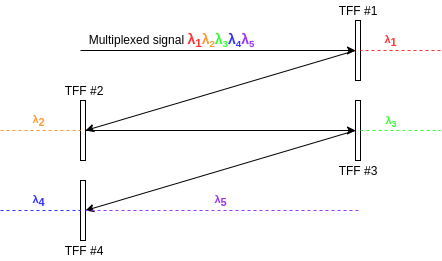
\includegraphics[scale=0.5]{demultiplexer.png}}
	\caption{Demultiplexing in WDM}
	\label{demultiplexing}
\end{figure}

\subsection{EONs}
Elastic optical network (EON) is a novel approach to optical networks, stemming from WDM systems. In WDM grid of spectrum resources is fixed, while in EON the grid is flexible, it changes to accommodate traffic. Channel spacing is also smaller, thus saving spectrum resources.

\section{Multicasting in WDM}

\section{Multicasting in EONs}

\begin{thebibliography}{00}
\bibitem{b1}
\end{thebibliography}
\end{document}
